\documentclass[conference]{IEEEtran}
\IEEEoverridecommandlockouts

\usepackage{cite}
\usepackage{amsmath,amssymb}
\usepackage{graphicx}
\usepackage{tikz}
\usetikzlibrary{arrows.meta,positioning,shapes.geometric}
\usepackage{booktabs}
\usepackage{url}

\graphicspath{{../benchmarks/}{./figures/}}

\newcommand{\taulow}{\tau_{\mathrm{low}}}
\newcommand{\tauhigh}{\tau_{\mathrm{high}}}
\newcommand{\sbar}{\bar{S}}

\begin{document}
\newcommand{\taulow}{\tau_{\mathrm{low}}}
\providecommand{\tauhigh}{\tau_{\mathrm{high}}}
\providecommand{\sbar}{\bar{S}}
\begin{figure}[t]
\centering
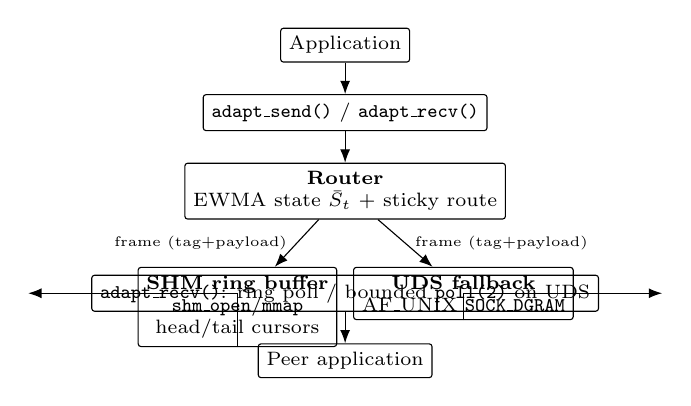
\begin{tikzpicture}[font=\scriptsize,>=Latex,
  box/.style={draw,rounded corners=1pt,align=center,inner sep=3pt},
  lbl/.style={font=\tiny,align=center}]
\node[box] (app) {Application};
\node[box,below=4mm of app] (api)
  {\texttt{adapt\_send()} / \texttt{adapt\_recv()}};
\node[box,below=4mm of api] (rt)
  {\textbf{Router}\\ EWMA state $\bar S_t$ + sticky route};
\node[box,below left=6mm and 1mm of rt.south] (shm)
  {\textbf{SHM ring buffer}\\ \texttt{shm\_open}/\texttt{mmap}\\
   head/tail cursors};
\node[box,below right=6mm and 1mm of rt.south] (uds)
  {\textbf{UDS fallback}\\ AF\_UNIX \texttt{SOCK\_DGRAM}};
\node[box,below=7mm of rt.south] (mux)
  {\texttt{adapt\_recv()}: ring poll / bounded \texttt{poll(2)} on UDS};
\node[box,below=4mm of mux] (peer) {Peer application};
\draw[->] (app) -- (api);
\draw[->] (api) -- (rt);
\draw[->] (rt) -- (shm)
  node[lbl,midway,left,align=right]{frame (tag+payload)};
\draw[->] (rt) -- (uds)
  node[lbl,midway,right,align=left]{frame (tag+payload)};
\draw[->] (shm.south) |- ([xshift=-8mm]mux.west);
\draw[->] (uds.south) |- ([xshift=8mm]mux.east);
\draw[->] (mux) -- (peer);
\end{tikzpicture}
\caption{AdaptIPC data flow through one endpoint. Every outbound message is
classified by the EWMA/hysteresis router of Fig.~\ref{fig:decision} and
transmitted either through the lock-free shared-memory ring buffer or the
AF_UNIX datagram fallback; each frame carries a one-byte transport tag.
The dashed edge is the escalation guard: an individual UDS-classified
message that exceeds the datagram ceiling is sent via SHM without moving
the sticky routing state. On the receiving side, the
\texttt{adapt\_recv()} multiplexer accepts whichever transport delivers
next (Section~IV-D).}
\label{fig:arch}
\end{figure}
\end{document}

